% A workaround to allow relative paths in included subfiles
% that are to be compiled separately
% See https://tex.stackexchange.com/questions/153312/subfiles-inside-a-subfile-using-relative-paths
\providecommand{\main}{..}
\documentclass[\main/thesis.tex]{subfiles}

\begin{document}

\chapter{Theoretical Results}


In this section, we consider the policy improvement guarantees, or lack thereof, for the reverse and forward KL. To the best of our knowledge, there is as yet only one with guarantees: the reverse KL when assuming exact minimization in each state \citep[Lemma 2]{haarnoja2018soft}. We first provide an extension of this result to rely only upon reverse KL minimization \textit{on average} across states. Next, we provide a counterexample where optimizing the forward KL \textit{does not} induce policy improvement.  Finally, we discuss further assumptions that can be made to ensure that forward KL does induce policy improvement.

\section{Reverse KL}
Throughout, we assume that the class of policies $\Pi$ consists of policies whose entropies are finite; this assumption is not restrictive for finite action-spaces as entropy is always finite in that setting. The assumption of finite entropies is necessary just to ensure that the soft value functions are well-defined. 

First, we note a strengthening of the original result for policy improvement under the reverse KL \citep{haarnoja2018soft}. By examining the proof of their Lemma 2, their new policy $\pi_{\mathrm{new}}$ does not have to minimize the reverse KL; rather, it suffices that $\pi_{\mathrm{new}}$ is smaller in reverse KL than $\pi_{\mathrm{old}}$ at every state $s$. 
\begin{lemma}[Policy Improvement under RKL Reduction, Restatement of Lemma 2 \citep{haarnoja2018soft}]\label{lem:stronger-sac}
For $\piold, \pinew \in \Pi$, if for all $s$
\begin{align*}
    \KL(\pinew(\cdot \mid s) \parallel \boltzmannQ^\piold_\tau(s, \cdot)) \le \KL(\piold(\cdot \mid s) \parallel \boltzmannQ_\tau^\piold(s, \cdot))\nonumber
\end{align*}
then $Q^\pinew_\tau(s, a) \geq Q^\piold_\tau(s, a)$ for all $(s, a)$ and $\tau > 0$.
\end{lemma}
\begin{proof}
Same proof as in \citet{haarnoja2018soft}.
\end{proof}
It turns out that a version of this result is true under expectation. First, however, it will be useful to note a ``soft'' counterpart to the classical performance difference lemma \citep{kakade2002approximately}. To state the performance difference lemma, we need to define some concepts. 
\begin{definition}[Performance Criterion]\label{def:perf-criterion}
For a start state distribution $\rho_0$, the performance criterion is defined to be
\begin{align*}
    \eta(\pi) := \Ex_{\rho_0}[V^\pi(s)].
\end{align*}
\end{definition}

\begin{definition}[State Visitation Distribution]\label{def:d_pi}
For a policy $\pi$ and starting state distribution $\rho$, the (future) state visitation distribution is defined as follows.
\begin{align*}
    d^\pi(s) := (1 - \gamma) \sum_{t = 0}^\infty \gamma^t \Pr(S_t = s \mid s_0 \sim \rho_0, \pi),
\end{align*}
where $\Pr(s_t = s \mid s_0 \sim \rho_0, \pi)$ is the probability of the $t$-th state with respect to the start state distribution and the trajectory induced by $\pi$. 
\end{definition}
Often in the literature, \Cref{def:d_pi} is defined without the additional $(1 - \gamma)$ term in front. This version is known as the \textit{unnormalized} visitation distribution.

\begin{definition}[Advantage]\label{def:advantage}
For any policy $\pi$, the \textit{advantage} is 
\begin{align*}
    A^\pi(s, a) := Q^\pi(s, a) - V^\pi(s).
\end{align*}
\end{definition}
The advantage asks, what is the average benefit if I take action $a$ in state $s$, as opposed to drawing an action from $\pi$?

The classical performance difference lemma is the following. 
\begin{lemma}[Performance Difference Lemma \citep{kakade2002approximately}]\label{lemma:perf-diff}
For any policies $\piold, \pinew$, we obtain the following relationship when using non-soft values, 
\begin{align*}
    \eta(\pinew) = \eta(\piold) + \frac{1}{1 - \gamma} \Ex_{d^{\pinew}, \pinew}[A^{\piold}(s, a)],
\end{align*}
where the notation $\Ex_{d^{\pinew}, \pinew}$ indicates the distributions for the states and actions, respectively 
\begin{equation*}
 \Ex_{d^{\pinew}, \pinew}[A^{\piold}(s, a)] \defeq \int_{\statespace} d^{\pinew}(s) \int_{\actionspace} \pinew(a | s) A^{\piold}(s,a) \ da \ ds.
\end{equation*}
%
\end{lemma}
\noindent Let's define the soft performance criterion. 
\begin{definition}[Soft Performance Criterion]\label{def:soft-performance}
The soft performance criterion is defined by the following, for a given temperature $\tau > 0$.
\begin{align*}
    \eta_\tau(\pi) := \Ex_{\rho_0}[V^\pi_\tau(s)].
\end{align*}
\end{definition}
It will also be helpful to have a soft version of the advantage. An intuition for the advantage in the non-soft setting is that it should be zero when averaged over $\pi$. To enforce this requirement in the soft setting, we require a small modification.
\begin{definition}[Soft Advantage]\label{def:soft-advantage}
For a policy $\pi$ and temperature $\tau > 0$, the soft advantage is
\begin{align*}
    % A^\pi_\tau(s, a) := Q^\pi_\tau(s, a) + \tau \entropy(\pi(\cdot \mid s)) - V^\pi_\tau(s).
    A^\pi_\tau(s, a) := Q^\pi_\tau(s, a) - \tau \log \pi(a \mid s) - V^\pi_\tau(s).
\end{align*}
\end{definition}
\noindent If $\tau = 0$, we recover the usual definition of the advantage function. It is also true that $\Ex_\pi[A^\pi_\tau(s, a)]= 0$, by definition of the soft value functions. We are ready for a soft performance difference lemma. 
\begin{lemma}[Soft Performance Difference]\label{lemma:soft-performance-difference}
For any policies $\piold, \pinew$, the following is true for any $\tau \geq 0$.
\begin{align*}
   &\eta_\tau(\pinew) - \eta_\tau(\piold) =\\
      &\quad \frac{1}{1 - \gamma}\Ex_{d^{\pinew}, \pinew}[A_\tau^{\piold}(s, a)] + \frac{\tau}{1 - \gamma} \Ex_{d^\pinew}[\KL(\pinew(\cdot \mid s) \parallel \piold(\cdot \mid s))].
%   &\quad \frac{1}{1 - \gamma}\Ex_{d^{\pinew}, \pinew}[A_\tau^{\piold}(s, a)] + \frac{\tau}{1 - \gamma} \Ex_{\pinew}[\entropy(\piold(\cdot \mid s)) - \entropy(\pinew(\cdot \mid s))]].
\end{align*}
\end{lemma}
\begin{proof}
%
The calculation is straightforward. When we write $\Ex$ without any subscripts, we mean the expectation over the trajectory distribution induced by $\rho_0$ and $\pinew$.
\begin{align*}
    \frac{1}{1 - \gamma}&\Ex_{d^{\pinew},\pinew}[A^{\piold}_\tau(s, a)]] = \Ex\left[\sum_{t = 0}^\infty \gamma^t A^{\piold}(s_t, a_t)\right]\\
    &\quad \triangleright \text{by definition of the visitation distribution}\\
    &= \Ex\left[\sum_{t = 0}^\infty \gamma^t (Q^\piold_\tau(s_t, a_t) - \tau \log \piold(\cdot \mid s_t) - V^{\piold}(s_t))\right]\\
    &\quad \triangleright \text{by definition of the soft advantage}\\
        &= \Ex\left[\sum_{t = 0}^\infty \gamma^t (r(s_t, a_t) + \gamma V_\tau^{\piold}(s_{t + 1}) - \tau \log \piold(\cdot \mid s_t) - V^{\piold}_\tau(s_t))\right]\\
        &\quad \triangleright \text{from expanding } Q^\piold_\tau \text{ and pulling the expectation outside}\\
        &= \Ex\left[\sum_{t = 0}^\infty \gamma^t (r(s_t, a_t) - \tau \log \piold(\cdot \mid s_t)) - V_\tau^{\piold}(s_0)\right]\\
        &\quad \triangleright \text{from the telescoping series } \gamma V^\piold_\tau(s_{t + 1}) - V^\piold_\tau(s_t)\\
        &= -\eta_\tau(\piold) + \Ex\left[\sum_{t = 0}^\infty \gamma^t (r(s_t, a_t) - \tau \log  \piold(\cdot \mid s_t)) \right]\\
        &\quad \triangleright \text{by definition of } \eta_\tau(\piold)\\
        &= -\eta_\tau(\piold) + \eta_\tau(\pinew) + \Ex\left[\sum_{t = 0}^\infty \gamma^t \tau (\log \pinew(\cdot \mid s_t) -  \log  \piold( \cdot \mid s_t)) \right] \\
        &\quad \triangleright \text{adding and subtracting } \tau \log \pinew(\cdot \mid s_t)\\
        &= -\eta_\tau(\piold) + \eta_\tau(\pinew)  + \frac{\tau}{1 - \gamma} \Ex_{d^{\pinew}}[\KL(\pinew(\cdot \mid s) \parallel \piold(\cdot \mid s))]
\end{align*}
\end{proof}
The presence of the extra KL term in \Cref{lemma:soft-performance-difference} is intriguing. Since the KL divergence is non-negative, one may be able improve upon $\eta_\tau(\piold)$ even with a negative advantage $A^\pi_\tau(s, a)$; the degree of this ``bonus'' is modulated by $\tau$. If we set $\tau = 0$, we recover the classical performance difference lemma. 

\begin{proposition}[Policy Improvement under Average RKL Reduction]\label{prop:avg-reverse-kl}
For $\piold, \pinew \in \Pi$, if
\begin{align}\label{eq:avg-rev-kl-policy-assumption}
    \Ex_{d^{\pinew}}&[\KL(\piold(\cdot \mid s) \parallel \boltzmannQ_\tau^{\piold}(s, \cdot))] \geq \Ex_{d^{\pinew}}[\KL(\pinew(\cdot \mid s) \parallel \boltzmannQ_\tau^{\piold}(s, \cdot))], \nonumber
\end{align}
then $\eta_\tau(\pinew) \geq \eta_\tau(\piold)$.

\end{proposition}
\begin{proof}
First, we calculate the KL inequality.
\begin{align*}
    &\Ex_{d^{\pinew}}[\KL(\piold(\cdot \mid s) \parallel \boltzmannQ_\tau^{\piold}(s, \cdot))] \geq \Ex_{d^{\pinew}}[\KL(\pinew(\cdot \mid s) \parallel \boltzmannQ_\tau^{\piold}(s, \cdot))]\\
    &\implies \Ex_{d^{\pinew}}[\Ex_{\piold}[\tau \log \piold(\cdot \mid s) - Q^{\piold}(s,\cdot)]] \\
    & \quad\quad\geq \Ex_{d^{\pinew}}[\Ex_{\pinew}[\tau \log \pinew(\cdot \mid s) - Q^{\piold}(s, \cdot)]]\\
    &\quad \triangleright \text{expanding the RKL definition and multiplying by } \tau\\
    &\implies -\Ex_{d^{\pinew}}[V^{\piold}(s)] \geq \Ex_{d^{\pinew}}[\Ex_{\pinew}[\tau \log \pinew(\cdot \mid s) - Q^{\piold}(s, \cdot)]\\
    &\quad \triangleright \text{because } V^\piold_\tau(s) = \Ex_\piold[Q^\piold_\tau(s, a) - \tau \log \piold(a \mid s)]\\
    &\implies \Ex_{d^{\pinew}, \pinew}[Q^{\piold}_\tau(s, a) - V^{\piold}_\tau(s)] \geq \tau \Ex_{d^{\pinew}, \pinew}[\log \pinew(\cdot \mid s)]\\
    &\quad \triangleright \text{rearranging}\\
    &\implies \Ex_{d^{\pinew}, \pinew}[A_\tau^{\piold}(s, a)] \geq \tau \Ex_{d^{\pinew}}[\KL(\pinew(\cdot \mid s) \parallel \piold(\cdot \mid s))]\\
    &\quad \triangleright \text{subtracting } \tau \Ex_{d^\pinew, \pinew}[\log \piold(\cdot \mid s) ] \text{ from both sides}
\end{align*}
%
Since the KL divergence is non-negative, the inequality we just derived implies that the RHS of \Cref{lemma:soft-performance-difference} is also non-negative. Hence, $\eta_\tau(\pinew) \geq \eta_\tau(\piold).$
\end{proof}
\noindent Note that we cannot set $\tau = 0$ in the above proof as we divide by $\tau$ in $\boltzmannQ$. 

We remark that the guarantee for \Cref{prop:avg-reverse-kl} is in terms of $\eta_\tau$, whereas the result in \Cref{lem:stronger-sac} is in terms of $Q^\pi_\tau$. The reason for this distinction is that in assuming an average KL reduction in \Cref{prop:avg-reverse-kl}, there does not seem to be a way to extract the action values on a per-state basis. Hence, the guarantee must of necessity be an average guarantee across states, rather than a guarantee for the value function at each state. 



% forward KL
\section{Forward KL}
Unfortunately, the same policy improvement properties do not hold unmodified for the forward KL. 
\begin{proposition}[Counterexample for Policy Improvement with FKL]\label{lem:forward-kl-counterexample}
There exists an MDP, a state $s'$, an initial policy $\piold$, policy $\pinew$, and temperature $\tau > 0$ such that for any $\gamma \in (0, 1]$
\begin{equation*}
    \forall s \in S,\, \KL(\boltzmannQ_\tau^\piold(s, \cdot) \parallel \piold(\cdot \mid s) \geq \KL(\boltzmannQ_\tau^\piold(s, \cdot) \parallel \pinew(\cdot \mid s))
    \end{equation*}
but $\forall a \in \actionspace, \, Q_\tau^\pinew(s', a) < Q_\tau^\piold(s', a)$.
\end{proposition}
\begin{proof}
Let us first construct the MDP. The MDP is episodic with two states and three actions in each state. $s_0$ is the start state, transitioning to state $s_1$ under any action, which then transitions to the terminal state under any action. The numbers near the arrows represent the reward upon taking the action corresponding to an arrow, from a state. From top to bottom, we have actions $a_0, a_1, a_2$. 

\begin{center}
\begin{tikzpicture}[auto,node distance=10mm,>=latex,font=\small]
    \tikzstyle{round}=[thick,draw=black,circle]

    \node[round] (s0) {$s_0$};
    \node[round,right=20mm of s0] (s1) {$s_1$};
    \node[round,rectangle,right=20mm of s1] (T) {$T$};

    \draw[->] (s0) -- node {0} (s1);
    \draw [->] (s0) to [out=30,in=150] node {-1} (s1);
    \draw [->] (s0) to [out=-30,in=210] node {1} (s1);
    \draw[->] (s1) --  node{0}(T);
    \draw [->] (s1) to [out=30,in=150] node{-2} (T);
    \draw [->] (s1) to [out=-30,in=210] node {1} (T);
    % \draw[->] (s0) [out=40,in=100,loop] to coordinate[pos=0.1](aa) (s0);
\end{tikzpicture}
\end{center}
%

Let our initial policy $\piold$ be the equiprobable policy for all states and actions. That is, $\forall\, (s, a)$, $\piold(a \mid s) = \frac{1}{3}$. Consider $\pinew$ to be the following. 
\begin{align*}
    \pinew(\cdot \mid s_0) &= \piold(\cdot \mid s_0)\\
    \pinew(a_0 \mid s_1) &= 3/8 \\
    \pinew(a_1 \mid s_1) &= 2/8\\
    \pinew(a_2 \mid s_1) &= 3/8
\end{align*}
%
Our strategy is the following: show that (1) $\pinew$ reduces the forward KL as it ``commits'' more at $s_1$, but that (2) $\piold$ has higher entropy and thus a higher soft action-value at $s_0$. A straightforward calculation provides the soft value functions of $\piold$ and $\pinew$ at $s_1$.
\begin{align*}
    V_\tau^\piold(s_1) &= -1/3  + \tau \ln 3    \\
    V_\tau^\pinew(s_1) &= -2 \cdot 3/8 + 3/8 + \tau \entropy(\pinew(\cdot \mid s_1)) = -3/8 + \tau\entropy(\pinew(\cdot \mid s_1))
\end{align*}
Recall that the soft action-value can be written as 
\begin{align*}
    Q_\tau^\pi(s, a) := r(s, a) + \gamma \Ex_{s'\sim p(\cdot \mid s, a)}[V^\pi(s)]. 
\end{align*}
Because this MDP is deterministic, we can rewrite the expectation above as the evaluation $V^\pi(s')$. The soft action-value of $\piold$ is 
\begin{align*}
    Q_\tau^\piold(s_0, a_0) &= -1 + \gamma \, V_\tau^\piold(s_1) = \gamma \,\tau \ln 3 - \frac{3 + \gamma}{3}  && Q_\tau^\piold(s_1, a_0) &= -2 \\
    Q_\tau^\piold(s_0, a_1) &= 0 +  \gamma\, V_\tau^\piold(s_1) = \gamma \,\tau\ln3 - \frac{\gamma}{3} && Q_\tau^\piold(s_1, a_1) &= 0 \\
    Q_\tau^\piold(s_0, a_2) &= 1 + \gamma\, V_\tau^\piold(s_1) = \frac{3 - \gamma}{3} + \gamma \,\tau\, \ln3 && Q_\tau^\piold(s_1, a_2) &= 1  
\end{align*}
%
The exponentiated action-value $\boltzmannQ_\tau$ is as follows.
\begin{align*}
    \boltzmannQ_\tau(s, a) := \frac{\exp(Q(s, a) \tau^{-1})}{\sum\limits_b \exp(Q(s, b) \tau^{-1})}
\end{align*}
%
The partition function at $s_1$ is given by the following.
\begin{align*}
    % Z(s_0) &:= \sum_a \exp(Q_\tau^{\piold}(s_0, a) \tau^{-1}) = \exp(\tau^{-1} V^\piold(s_1))(1 + \exp(\tau^{-1}) + \exp(-\tau^{-1})), \\
    Z(s_1) &:= \sum_a \exp(Q_\tau^{\piold}(s_1, a) \tau^{-1}) = 1 + \exp(\tau^{-1}) + \exp(-2\tau^{-1}).
\end{align*}
Calculating the exponentiated soft action-values at $s_1$,
\begin{align*}
    % \boltzmannQ_\tau^\piold(s_0, a_0) &= \frac{\exp(-\tau^{-1} + \tau^{-1}V^\piold(s_1) )}{Z(s_0)} &= \frac{\exp(-\tau^{-1})}{1 + \exp(\tau^{-1}) + \exp(-\tau^{-1})}, \\
    % \boltzmannQ_\tau^\piold(s_0, a_1) &= \frac{\exp(\tau^{-1}V^\piold(s_1) )}{Z(s_0)} &= \frac{1}{1 + \exp(\tau^{-1}) + \exp(-\tau^{-1})}, \\
    % \boltzmannQ_\tau^\piold(s_0, a_2) &= \frac{\exp(\tau^{-1} + \tau^{-1}V^\piold(s_1) )}{Z(s_0)} &= \frac{\exp(\tau^{-1})}{1 + \exp(\tau^{-1}) + \exp(-\tau^{-1})},  \\
    \boltzmannQ_\tau^\piold(s_1, a_0) &= \frac{\exp(-2\tau^{-1})}{1 + \exp(\tau^{-1}) + \exp(-2\tau^{-1})},\\
    \boltzmannQ_\tau^\piold(s_1, a_1) &= \frac{1}{1 + \exp(\tau^{-1}) + \exp(-2\tau^{-1})},\\
    \boltzmannQ_\tau^\piold(s_1, a_2) &= \frac{\exp(\tau^{-1})}{1 + \exp(\tau^{-1}) + \exp(-2\tau^{-1})}.
\end{align*}
The new soft action-value at $s_0$ is given by
\begin{align*}
    Q_\tau^\pinew(s_0, a_0) &= -1 + \gamma \, V^\pinew_\tau(s_1) \\
        &= -1 - \frac{3\gamma}{8} + \gamma\, \tau\, \entropy(\pinew(\cdot \mid s_1)) \\
        &= \frac{-8 - 3 \gamma}{8} + \gamma\, \tau\, \entropy(\pinew(\cdot \mid s_1)),\\
    Q_\tau^\pinew(s_0, a_1) &= - \frac{3\, \gamma }{8} + \gamma\, \tau\,\entropy(\pinew(\cdot \mid s_1)) ,\\
    Q_\tau^\pinew(s_0, a_2) &= \frac{8 - 3\gamma}{8} + \gamma\, \tau\, \entropy(\pinew(\cdot \mid s_1))
\end{align*}

Let's now compare $Q_\tau^\pinew$ and $Q_\tau^\piold$. Note that entropy is maximized by a uniform distribution, so $\tau \,\entropy(\pinew(\cdot \mid s_1)) < \tau \ln 3$, regardless of the value of $\tau > 0$ and $\gamma > 0$. Let's put the reward terms under a common denominator. 
\begin{align*}
    Q^\piold_\tau(s_0, a_0) - Q^\pinew_\tau(s_0, a_0) &> - \frac{3 + \gamma}{3} + \frac{8 + 3 \gamma}{8} &= \frac{\gamma}{24},\\
    Q^\piold_\tau(s_0, a_1) - Q^\pinew_\tau(s_0, a_1) &> - \frac{\gamma}{3} + \frac{3\, \gamma }{8}  &= \frac{\gamma}{24},\\
    Q^\piold_\tau(s_0, a_2) - Q^\pinew_\tau(s_0, a_2) &> \frac{3 - \gamma}{3} - \frac{8 - 3 \gamma}{8} &= \frac{\gamma}{24}.
\end{align*}
% We also have the following. 
% \begin{align*}
%     -11/8 &< -4/3\\
%     -3/8 &< -1/3\\
%     5/8 &< 2/3
% \end{align*}
Thus, for any $\gamma \in (0, 1]$, $Q_\tau^\pinew(s_0, a) < Q_\tau^\piold(s_0, a)$ for all actions $a$. 

% Let's now set $\tau = 1$. 
Let's now compare the forward KL divergences. Because the policies are the same at $s_0$, we have 
\begin{align*}
    \KL(\boltzmannQ_\tau^\piold(s_0, \cdot) \parallel \pinew(\cdot \mid s_0)) &= \KL(\boltzmannQ_\tau^\piold(s_0, \cdot) \parallel \piold(\cdot \mid s_0)).
\end{align*}
Calculating the rest of the forward KL divergences,
\begin{align*}
    % \KL(\boltzmannQ_\tau^\piold(s_0, \cdot) \parallel \piold(\cdot \mid s_0)) &= -\entropy(\boltzmannQ_\tau^\piold(s_0, \cdot)) - \frac{1}{Z(s_1)} (\exp(-1) \log(1/3) + \log(1/3) + \exp(1) \log(1/3))  \\
    &\KL(\boltzmannQ_\tau^\piold(s_1, \cdot) \parallel \piold(\cdot \mid s_1)) =\\
    &\quad-\entropy(\boltzmannQ_\tau^\piold(s_1, \cdot)) - \log(1/3) \frac{\exp(-2\tau^{-1}) + 1 + \exp(\tau^{-1})}{1 + \exp(\tau^{-1}) + \exp(-2\tau^{-1})}   \\
    &\KL(\boltzmannQ_\tau^\piold(s_1, \cdot) \parallel \pinew(\cdot \mid s_1)) =\\
    &\quad-\entropy(\boltzmannQ_\tau^\piold(s_1, \cdot)) - \frac{\exp(-2\tau^{-1}) \log(3/8)+ \log(2/8) + \exp(\tau^{-1}) \log(3/8)}{1 + \exp(\tau^{-1}) + \exp(-2\tau^{-1})}   
\end{align*}
In order to have $\KL(\boltzmannQ_\tau^\piold(s_1, \cdot) \parallel \piold(\cdot \mid s_1)) > \KL(\boltzmannQ_\tau^\piold(s_1, \cdot) \parallel \pinew(\cdot \mid s_1))$, it is sufficient and necessary to have
\begin{align*}
    &- \log(1/3) \frac{\exp(-2\tau^{-1}) + 1 + \exp(\tau^{-1})}{1 + \exp(\tau^{-1}) + \exp(-2\tau^{-1})} \\
    &\quad > - \frac{\exp(-2\tau^{-1}) \log(3/8)+ \log(2/8) + \exp(\tau^{-1}) \log(3/8)}{1 + \exp(\tau^{-1}) + \exp(-2\tau^{-1})}.
\end{align*}
Or, after simplifying,
\begin{align*}
    &- \log(1/3) (\exp(-2\tau^{-1}) + 1 + \exp(\tau^{-1})) \\ 
    &\quad > - (\exp(-2\tau^{-1}) \log(3/8)+ \log(2/8) + \exp(\tau^{-1}) \log(3/8))\\
    &\iff \exp(-2\tau^{-1})(\log(3/8) - \log(1/3)) + \log(2/8) - \log(1/3)\\
    &\quad\quad+ \exp(\tau^{-1})(\log(3/8) - \log(1/3)) > 0\\
    &\iff \exp(-2\tau^{-1})\log(9/8) + \log(3/4) + \exp(\tau^{-1})\log(9/8) > 0\\
    &\iff \log(9/8) + \log(3/4)\exp(2 \tau^{-1}) + \exp(3\tau^{-1})\log(9/8) > 0.
\end{align*}
Setting $y = \exp(\tau^{-1})$, we are interested in the cubic inequality
\begin{align*}
    \log(9/8) + \log(3/4) y^2 + y^3\log(9/8) > 0.
\end{align*}
Noting that the leading term of the cubic is positive, there must be some $y_0$ such that for $y > y_0$, the inequality above holds. This $y_0$ must be the largest root of the cubic expression. A root-solver gives $y_0 > 2.25$, so the above inequality holds for $\exp(\tau^{-1}) = y > 2.25$, or in other words for $1.23 \approx \frac{1}{\log 2.25} > \tau$.

\end{proof}
%
\Cref{lem:forward-kl-counterexample} shows that there is an MDP and two policies in which one policy $\pinew$ can have a lower FKL, but fail to be a better policy for small enough $\tau$. It might seem like \Cref{lem:forward-kl-counterexample} could contradict the RKL improvement result in \Cref{lem:stronger-sac}, but \Cref{lem:forward-kl-counterexample} is a statement about a particular policy, and not about any policy that reduces the RKL.

From examining the proof of \Cref{lem:forward-kl-counterexample}, it might also be surprising that the result holds for sufficiently small $\tau$. That is, for $\tau < \tau_0$, for some $\tau_0$, there will always be a policy that reduces the FKL, but that has strictly worse performance than the previous policy. Such a result might seem unintuitive since one would expect that the more one reduces the FKL, the better the policy should be, given that the FKL is minimized by setting the subsequent policy to be exactly the target distribution. Nevertheless, such reasoning says nothing about the path of policies to the superior, target distribution policy. 

A natural question is if this counterexample is pathological. Since reducing the FKL to 0 corresponds to reducing the RKL to 0 (i.e., setting $\pinew = \boltzmannQ^\piold_\tau$), it seems plausible that if the FKL is reduced enough, the new policy $\pinew$ will be better. One may also wonder if by selecting a temperature judiciously enough, optimizing for the forward KL might induce policy improvement. With some qualifications, the answer is in the positive. 
%
\begin{proposition}[Policy Improvement for FKL with Sufficient Reduction]\label{prop:forward-kl-surrogate-2}
Assume a discrete action space with $|\actionspace| < \infty$, with a policy space $\Pi$ that consists of policies where $\pi(a \mid s) > 0$ for all $a$. Let $C$, $\piold, \pinew \in \Pi$ be such that for a state $s$,
\begin{align}\label{eq:forward-improvement}
    \KL(\boltzmannQ^{\piold}(s, \cdot) \parallel \pinew (\cdot \mid s)) + C \leq \KL(\boltzmannQ^{\piold}(s, \cdot) \parallel \piold(\cdot \mid s)),
\end{align}
where $C$ additionally satisfies
\begin{align*}
    C &\geq  \frac{1}{2}\sum_a  \left(1 - \frac{1}{\piold(a \mid s)}\right)^2 \left(1 + \frac{Q^\piold(s, a)}{\tau} + \frac{\exp(\tau^{-1} Q^\piold(s, a)) Q^\piold(s, a)^2}{2\tau^2}\right) \\
    &\quad + \frac{1}{2} \sum_a \exp(\tau^{-1} Q^\piold(s, a)) \tau^{-2} Q^\piold(s, a)^2 (1 - \piold(a \mid s))
\end{align*}
with $\tau > 0$. Then,
\begin{align*}
    \sum_a Q^{\piold}(s, a) \piold(a \mid s) \leq \sum_a Q^{\piold}(s, a) \pinew(a \mid s). 
\end{align*}
\end{proposition}
\begin{proof}

For the steps below, we will need to consider shifted, positive values $Q^{\piold}(s, a) + b $ where $b \defeq \max(0, -\min_{a \in \actionspace} Q^{\piold}(s,a)) + 0.01$. This shift does not affect \Cref{eq:forward-improvement} because the Boltzmann function is invariant to shifts in the logits. 
It suffices to focus on a single state $s$. We will suppress dependence on this state for notational simplicity. Let $\pi(a) \defeq \piold(a | s)$ and $Q(a) \defeq Q^{\piold}(s, a) + b > 0$. After cancelling the common entropy term and multiplying both sides by the partition function, \Cref{eq:forward-improvement} yields
\begin{align}\label{eq:first-ineq}
    \sum_a \exp(\tau^{-1} Q(a)) \log \frac{1}{\pinew(a)} + C \leq \sum_a \exp(\tau^{-1} Q(a)) \log \frac{1}{\piold(a)}.
\end{align}
For $x \geq 0$, we have $1 + x \leq \exp(x)$ and for $x \in (0, 1)$ we have $ \log \frac{1}{x} = -\log(x) \geq 1 - x$. Since we assumed $Q(a) > 0$ and $\piold$, $\pinew$ are not deterministic, these inequalities may be applied. Applying them to \Cref{eq:first-ineq} gives
\begin{align}\label{eq:second-ineq}
    \sum_a (1 + \tau^{-1} Q(a)) (1 - \pinew(a)) + C \leq \sum_a \exp(\tau^{-1} Q(a)) \log\frac{1}{\piold(a)}.
\end{align}
To get any further, we proceed by Taylor expansion. We will expand $\exp(x)$ around $x = 0$ and $\log (x)$ around $x = 1$. Now, using the Lagrange form of the remainder of Taylor expansions yields
\begin{align*}
    \exp(\tau^{-1} Q(a)) &= 1 + \tau^{-1} Q(a) + \frac{1}{2}\exp(\xi_a) \tau^{-2} Q(a)^2,\\
    \implies \exp(\tau^{-1} Q(a)) &\leq 1 + \tau^{-1} Q(a) + \frac{1}{2}\exp(\tau^{-1} Q(a)) \tau^{-2} Q(a)^2,\\
    \log(\piold(a)) &= \piold(a) - 1 - \frac{1}{2\kappa_a^2} (\piold(a) - 1)^2,\\
    \implies \log \frac{1}{\piold(a)} &= 1 - \piold(a) + \frac{1}{2\kappa_a^2} (\piold(a) - 1)^2\\
    \implies \log \frac{1}{\piold(a)} &\leq 1 - \piold(a) + \frac{1}{2\piold(a)^2} (\piold(a) - 1)^2\\
    \implies \log \frac{1}{\piold(a)} &\leq 1 - \piold(a) + \frac{1}{2} \left(1 - \frac{1}{\piold(a)}\right)^2
\end{align*}
for some $\xi_a \in (0, \tau^{-1}Q(a))$ and $\kappa_a \in (\piold(a), 1)$. 
Using the inequalities on the RHS of \Cref{eq:second-ineq} yields the following. 
\begin{align*}
    &\sum_a \exp(\tau^{-1} Q(a)) \log\frac{1}{\piold(a)}\\
    &\hspace{2em} \leq \sum_a (1 + \tau^{-1} Q(a))(1 - \piold(a)) + \mathbf{X},
\end{align*}
where $\mathbf{X}$ represents terms we have neglected for the moment. From re-examining \Cref{eq:second-ineq}, noting that $\sum_a (1 - \piold(a)) = \sum_a (1 - \pinew(a))$, and canceling out $\sum_a \tau^{-1} Q(a)$ on both sides, we have
\begin{align*}
    -\sum_a \tau^{-1}Q(a) \pinew(a) + C &\leq -\sum_a \tau^{-1}Q(a) \piold(a) + \mathbf{X}\\
    C -\mathbf{X} &\leq \tau^{-1} \sum_a Q(\pinew(a) - \piold(a))
\end{align*}

Notice that 
\begin{align*}
\sum_a Q(a)\pinew(a) &= \sum_a (Q^{\piold}(s, a) + b )\pinew(a) \\
&=  \sum_a Q^{\piold}(s, a) \pinew(a) +  b \sum_a \pinew(a) \\
&= \sum_a Q^{\piold}(s, a) \pinew(a) +  b \\
\implies  \sum_a Q(a)(\pinew(a) - \piold(a)) &=  \sum_a Q^{\piold}(s,a)(\pinew(a) - \piold(a))
\end{align*}
%
Therefore, to show that $\sum_a Q^{\piold}(s,a)\pinew(a) \ge \sum_a Q^{\piold}(s,a)\piold(a)$, it suffices that $C -\mathbf{X} \geq 0$, or equivalently that $C \geq \mathbf{X}$. 
\begin{align*}
    \mathbf{X} &:=  \frac{1}{2}\sum_a  \left(1 - \frac{1}{\piold(a)}\right)^2 (1 + \tau^{-1} Q(a) + \frac{1}{2}\exp(\tau^{-1} Q(a)) \tau^{-2} Q(a)^2) \\
    &\quad + \frac{1}{2} \sum_a \exp(\tau^{-1} Q(a)) \tau^{-2} Q(a)^2 (1 - \piold(a))
\end{align*}
Noting that every term is non-negative by assumption, the conclusion follows.
\end{proof}
The conclusions of \Cref{prop:forward-kl-surrogate-2} hold if $C$ is large enough; as $\tau$ decreases, $C$ must be larger, which explain the failure of policy improvement in \Cref{lem:forward-kl-counterexample}. On the other hand, if $\tau$ is large, then the requirement for $C$ becomes less onerous, although the resulting conclusion might be quite weak; soft action-values for large $\tau$ become dominated by the entropy term, weighing much less the contribution of reward from the environment. 

How large can the minimal $C$ required get? Using the MDP of \Cref{lem:forward-kl-counterexample}, in \Cref{fig:prop3-c} we plot the minimal $C$ as a function of temperature. The minimal $C$ is in fact larger than $\KL(\boltzmannQ^\piold(s_1, \cdot) \parallel \piold(\cdot \mid s_1))$! This suggests that the minimal $C$ is in fact an overestimate, which seems due to the looseness of the bounds, $\log x \leq x - 1$ in particular, we used in deriving it. 
\begin{figure}[!htb]
    \centering
    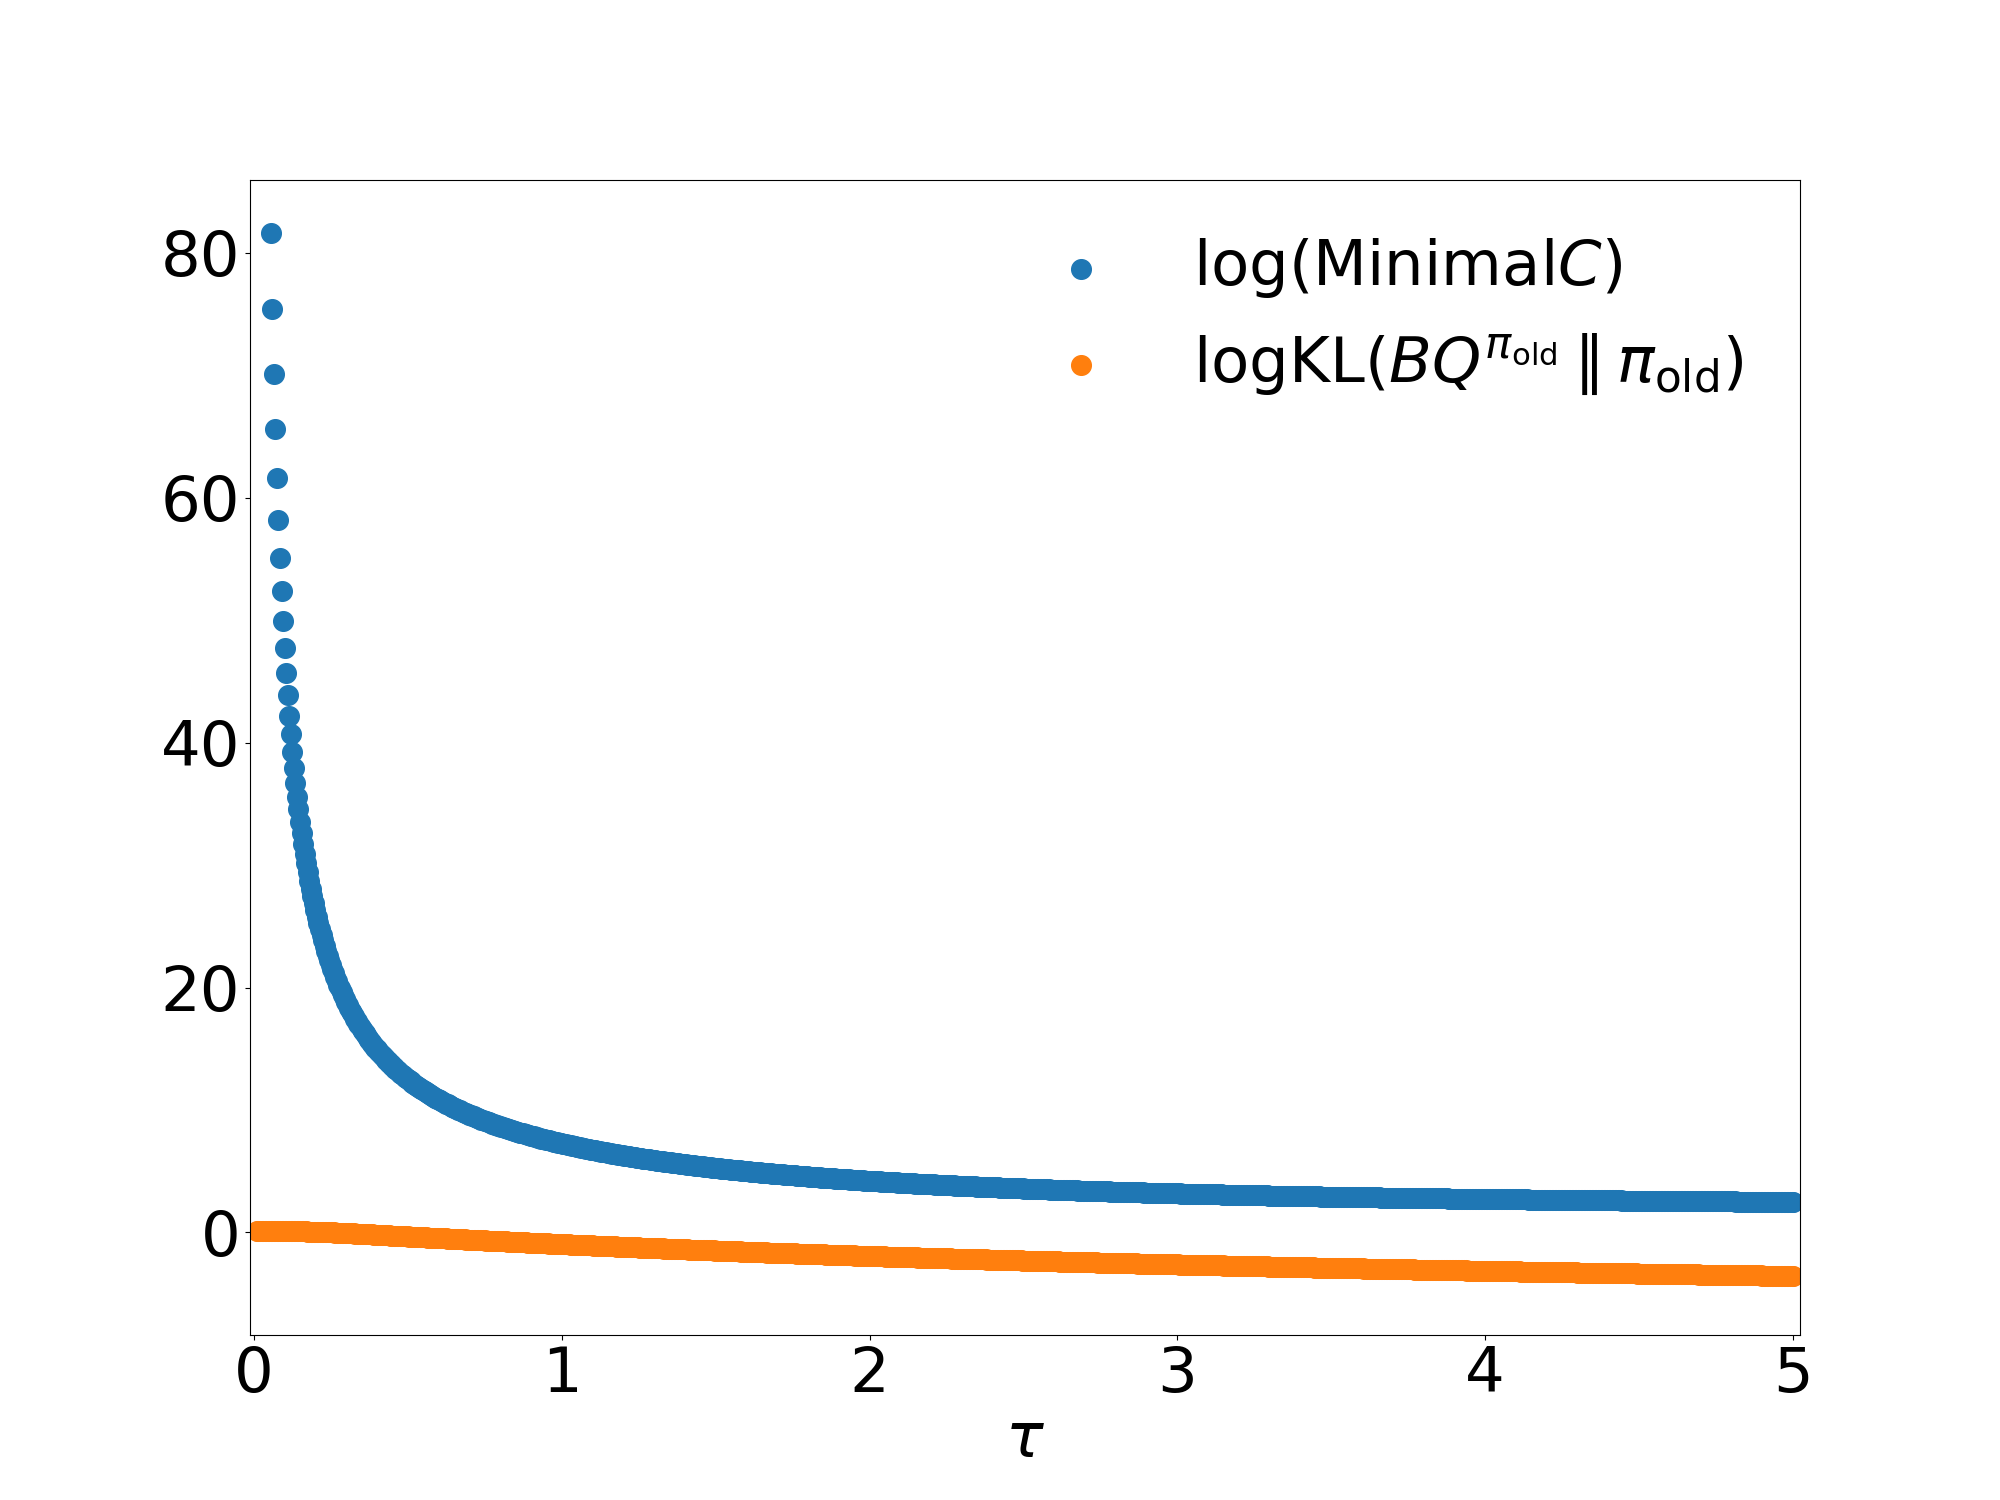
\includegraphics[width=\linewidth]{figs/theory/prop3.png}
    \caption{The minimal $C$ in \Cref{prop:forward-kl-surrogate-2} as a function of $\tau$, plotted against the KL divergence between $\boltzmannQ^\piold$ and $\piold$ at $s_1$ of the MDP in \Cref{lem:forward-kl-counterexample}.}
    \label{fig:prop3-c}
\end{figure}

If the conclusions of \Cref{fig:prop3-c} do hold across all states, and with an additional assumption, we can guarantee policy improvement. 
\begin{corollary}\label{cor:fkl-pi}
If 
\begin{align*}
    \Ex_{d^\pinew, \piold}[ Q^\piold_\tau(s, a)]\leq \Ex_{d^\pinew, \pinew}[Q^\piold_\tau(s, a)],
\end{align*}
and if 
\begin{align*}
    \tau \Ex_{d^\pinew}[\entropy(\pinew(\cdot \mid s))] \geq \tau \Ex_{d^\pinew}[\entropy(\piold(\cdot \mid s))],
\end{align*}
then $\eta_\tau(\pinew) \geq \eta_\tau(\piold)$. This conclusion also holds for $\tau = 0$.
\end{corollary}
\begin{proof}
If $\tau = 0$, then $\sum_a \piold(a \mid s) Q^{\piold}(s, a) = V^{\piold}(s)$. If the above holds for all states $s$, then $V^{\piold}(s) \leq \sum_a Q^{\piold}(s, a) \pinew(a \mid s)$ for all states and so $V^{\pinew} \geq V^{\piold}$ by the classical policy improvement theorem \citep{sutton2018reinforcement}. It follows that $\eta(\pinew) \geq \eta(\piold)$.

If $\tau > 0$, we may use \Cref{lemma:soft-performance-difference}, the soft performance difference lemma. Note that since we are working with soft value functions, we have the following relation between the soft state-value and the soft action-value. 
\begin{align*}
    \sum_a Q_\tau^\piold(s, a) \piold(a \mid s) = V_\tau^\piold(s) - \tau \entropy(\piold(\cdot \mid s)).
\end{align*}
Using the first assumption of the Corollary,
\begin{align*}
    \Ex_{d^\pinew, \piold}[V_\tau^\piold(s) + \tau \log\piold(\cdot \mid s)] &= \Ex_{d^\pinew, \piold}[ Q_\tau^\piold(s, a)] \\
    &\leq \Ex_{d^\pinew, \pinew}[ Q_\tau^\piold(s, a)].
\end{align*}
Rearranging and taking expectations, we have
\begin{align*}
    \Ex_{d^\pinew, \pinew}[Q_\tau^\piold(s, a) -& V_\tau^\piold(s)] \geq \tau \Ex_{d^\pinew, \piold}[\log \piold(\cdot \mid s)],\\
    \Ex_{d^\pinew, \pinew}[A_\tau^\piold(s, a)] &\geq \tau \Ex_{d^\pinew}[\Ex_{\piold}[\log \piold(\cdot \mid s)] - \Ex_{\pinew}[\log \piold(\cdot \mid s)]].\\
    &\quad \triangleright \text{adding } -\tau \Ex_{d^\pinew, \pinew}[\log \piold(\cdot \mid s)] \text{ to both sides}
\end{align*}
From Gibbs's inequality, the entropy of any distribution is strictly less than the cross-entropy of that distribution with any other distribution. In other words,
\begin{align*}
    \entropy(\pinew(\cdot \mid s)) &\leq \entropy(\pinew(\cdot \mid s), \piold(\cdot \mid s))\\
    -\Ex_\pinew[\log \pinew(\cdot \mid s)] &\leq - \Ex_\pinew[\log \piold(\cdot \mid s))]
\end{align*}
% \begin{align*}
%     \entropy(\piold(\cdot \mid s)) &\leq \entropy(\piold(\cdot \mid s), \pinew(\cdot \mid s))\\
%     -\Ex_\piold[\log \piold(\cdot \mid s)] &\leq - \Ex_\piold[\log \pinew(\cdot \mid s))]
% \end{align*}
Applying this inequality,
\begin{align*}
    \Ex_{d^\pinew, \pinew}[A_\tau^\piold(s, a)] &\geq \tau \Ex_{d^\pinew}[\Ex_{\piold}[\log \piold(\cdot \mid s)] - \Ex_{\pinew}[\log \pinew(\cdot \mid s)]]\\
    &= \tau \Ex_{d^\pinew}[ \entropy (\pinew(\cdot \mid s)) - \entropy(\piold(\cdot \mid s))]\\
    &\geq 0\\
    &\quad \triangleright \text{by the entropy assumption of the Corollary}
\end{align*}
%     &\geq\tau \Ex_{d^\pinew, \pinew}[\log \pinew(\cdot \mid s)] - \tau \Ex_{d^\pinew, \pinew}[\log \piold(\cdot \mid s)]\\
%     &\quad \triangleright \text{using the assumption in the Corollary}\\
%     &= \tau \Ex_{d^\pinew}[\KL(\pinew(\cdot \mid s) \parallel \piold(\cdot \mid s)]]
% \end{align*}
% Hence, the RHS of \Cref{lemma:soft-performance-difference} is non-negative, meaning that $\eta_\tau(\pinew) \geq \eta_\tau(\piold)$.
% To show that $\eta_\tau(\pinew) \geq \eta_\tau(\piold)$ with \Cref{lemma:soft-performance-difference}, it suffices to verify that
% \begin{align*}
%     \Ex_{d^\pinew, \pinew}[A_\tau^\piold(s, a)] \geq -\tau \Ex_{d^\pinew}[\KL(\pinew(\cdot \mid s) \parallel \piold(\cdot \mid s))].
% \end{align*}
% It will therefore suffice to show that
% \begin{align*}
%     &\tau \Ex_{d^\pinew}[\Ex_{\piold}[\log \piold(\cdot \mid s)] - \Ex_{\pinew}[\log \piold(\cdot \mid s)]] \\
%     &\quad\geq -\tau \Ex_{d^\pinew}[\KL(\pinew(\cdot \mid s) \parallel \piold(\cdot \mid s))].
% \end{align*}
% Let's write out the KL divergence.
% \begin{align*}
%     -\tau\Ex_{d^\pinew}[\KL(\pinew(\cdot \mid s) &\parallel \piold(\cdot \mid s))] \\
%     &= \tau\Ex_{d^\pinew}[\entropy(\pinew(\cdot \mid s))  + \Ex_\pinew[\log \piold(\cdot \mid s)]]\\
%     &\leq \tau \Ex_{d^\pinew}[\entropy(\piold(\cdot \mid s)) + \Ex_\pinew[\log \piold(\cdot \mid s)]]\\
%     &\quad \triangleright \text{from the entropy assumption in the Corollary}\\
%     &= \tau \Ex_{d^\pinew}[ \Ex_\pinew[\log \piold(\cdot \mid s)] - \Ex_\piold[\log \piold(\cdot \mid s)] ]\\
%     &\quad \triangleright \text{expanding the definition of entropy}
% \end{align*}
% The claim follows. 
\end{proof}
% \noindent The entropy assumption in \Cref{cor:fkl-pi} does not seem unreasonable; it only requires that $\pinew$ ``commit'' more than $\piold$. This ``committing'' seems natural to occur, as $\pinew$ hopefully selects actions with higher action-value more often than $\piold$.
\noindent The entropy assumption in \Cref{cor:fkl-pi} is a bit strange; for $\pinew$ to be better, it must ``commit'' less to actions, the opposite of what we would expect a policy to do when learning optimal actions. 

\section{Summary}
Here are some takeaways of the above discussion. 
\begin{enumerate}
    \item The RKL has a stronger policy improvement result than the FKL as it requires only that the RKL of $\pinew$ be no greater than the RKL of $\piold$.
    \item The FKL can fail to induce policy improvement, but this failure is linked to a temperature that is too low and/or an insufficient reduction in the FKL. For a large enough reduction and large enough temperature, coupled with an additional entropy assumption, policy improvement follows. 
\end{enumerate}


There are some limitations of this theory. We had to assume a finite action space for \Cref{prop:forward-kl-surrogate-2}. The reason here was to ensure that we could sensibly manipulate the remainder terms in the Taylor expansions. A general treatment of action spaces would at least require some work into the measurability and integrability of such terms as a function of the action. Moreover, the theory developed in this chapter is under ideal settings, assuming in particular access to the true value functions. For \Cref{prop:forward-kl-surrogate-2,cor:fkl-pi}, the looseness of the bounds we employed resulted in extremely strong sufficient conditions for FKL policy improvement. As we will see in our experiments, the FKL is often able to induce policy improvement in practice, suggesting a gap between the theory developed and the practical performance. 


\end{document}